\section{Let Míčku}
\label{ssec:let-micku}
Let míčku se často zjednodušuje a zanedbávají se některé síly, které na letící
míček působí. Když uvážíme jen gravitaci zjistíme, že by míček za letu měl
dráhou opsat parabolu. Pro kratší dobu letu a velkou rychlost tento předpoklad
není nikterak škodlivý.\footnote{Jako tomu bývá často právě ve stolním tenisu}.
Tyto síly můžeme vidět na rovnici \myref{rovnici}{eq:Newton} a na
\myref{obrázku}{fig:let-micku}.

\myref{Rovnice}{eq:Newton} získáme, když si rozepíšeme 2. Newtonův kinematický
zákon. 
\begin{equation}
 \label{eq:Newton}
 \textcolor{teal}{\vec{F_g}} + \textcolor{velcol}{\vec{v}} +
 \textcolor{drcol}{\vec{F_d}} + \textcolor{spcol}{\vec{F_m}} = m \vec{a}
\end{equation}

Již zmíněné síly budou v této sekci podrobněji popsány.

\begin{figure}[htbp]
 \centering
 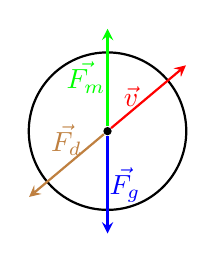
\begin{tikzpicture}
	%giganteska bola de fuego
	\node[fill=black,circle,inner sep=0pt, minimum size=3pt](center) at (0,0)
	{};
 \draw[thick] (center) circle (1);


	%speed
	\draw[thick, red, -stealth] (center) -- node[midway, left] {$\vec{v}$} (40:1.3);

	%gravitace
	\draw[thick, blue, -stealth] (center) --node[midway,right=-3pt] {$\vec{F_g}$} (-90:1.3);

	%drag
	\draw[thick,brown, -stealth] (center) --node[midway,left,above] {$\vec{F_d}$}
	 (220:1.3);

	%magnus force
	\draw[thick,green,-stealth] (center) --node[left=-3pt,midway] {$\vec{F_m}$} (90:1.3);


\end{tikzpicture}


 \caption{Síly působící na míček v letu}
 \label{fig:let-micku}
\end{figure}


\subsection{Rychlost}
\label{ssec:rychlost}
Rychlost (\speed{}), jako derivace polohy je jádrem samotného pohybu
(bez změny polohy není pohyb). Ze začátku dáme míčku nějakou energii a tím ho
uvedeme v pohyb.

Jakmile je ve vzduchu, působí na něj ostatní síly a ovlivňují jeho energii.
V případě, kterým se budeme zabívat, většina sil disipuje energii míčku. Jediný
jev, který by mohla prodlužovat dobu letu (tedy přidávat míčku energii) je jev
Magnusův. Tomu je věnována \myref{podsekce}{ssec:magnusova-sila}.


\subsection{Gravitační síla}
\label{ssec:gravitacni-sila}

Gravitační nebo také tíhová síla (\textcolor{grcol}{$F_g$}) je hned po rychlosti
nejdůležitější sílou v průběhu pohybu míčku. A spolu s rychlostí nejviditelněji
tvoří rajektorii míčku.

Gravitace je také nejjednoduší na modelování. Dokud můžeme pro celou trajektorii
považovat Zemi za lokálně plochou, gravitační síla míří vždy směrem kolmů dolů.
Také její amplituda bývá většinou konstantní, protože není časté, že by míček
během letu měnil svojí váhu a změna v nadmořské výšce je zpravidla zanedbatelná.

Matematicky můžeme velikost gravitační síly vyjádřit jako:
\[
 \textcolor{grcol}{F_g} = G\frac{m}{h}
\]
Kde $G$ je gravitační konstanta, $m$ je váha míčku a $h$ je nadmořská výška.

Z této rovnice je ještě jednodušší nahlédnout na fakt, že gravitační síla je pro
náš případ konstantní. 


\subsection{Odpor vzduchu}
\label{ssec:odpor-vzduchu}

Odpor vzduchu (\textcolor{drcol}{$F_d$}) je často zanedbáván a to kvůli své
relativní složitosti oproti již zmíněné gravitační síle. Odpor vzduchu je totiž
obecně závyslí na rychlosti a ploše, která aktivně do vzduchu naráží. V případě
míčku se mění jen rychlost stále se ovšem jedná o složitou sílu na implementaci.

Směr odporu vzduchu je vždy opačný ke směru pohybu jak můžeme vidět na
\myref{obrázku}{fig:let-micku}. Velikost odporu závysí
kromě dalších koeficientů hlavně na kvadrátu rychlosti. 


\subsection{Magnusova síla}
\label{ssec:magnusova-sila}

Magnusova síla (\textcolor{spcol}{$F_m$}) vzniká díky rotaci a vzájemnému tření
mezi míčkem a vzduchem (předpokládáme vzduch bez vlastní rychlosti). Směr magnusovy síly na \myref{obrázku}{fig:let-micku} je
specifický pro aktuální případ. Směr Magnusovi síly závisý na úhlové rychlost
(\spin{1}). Jestliže \spin{1}$<0$ tak Magnusova síla míří směrem nahoru a v
opačném případě dolů.

Intuitivním vysvětlením tohoto fenoménu je, že rotací míček tlačí směrem nahoru,
respektive dolů, a z 3. Newtonova zákonu tedy rozumíme, že vzduch naopak tlačí
míček dolů, respektive nahoru.

